\section{Koordinatensysteme und Koordinatentransformationen}

Um ein Modellauto steuern zu können, werden unter anderem die Informationen über den aktuellen Standort und den Zielpunkt, den das Fahrzeug ansteuern soll, benötigt. Die Trajektorie ist wiederum davon abhängig, an welcher Stelle sich die Fahrbahnmarkierungen befinden. Alle Positionen von Objekten im Raum werden deshalb mit Entfernungen relativ zu entsprechenden Koordinatensystemen beschrieben. Für die Beschreibung unseres TUCar auf dem Parcour und die Lage der Straßenlinien eignet sich das kartesische Koordinatensystem besser als Polar- oder Kugelkoordinaten. Letztendlich wurden drei hierarchisch angeordnete Koordinatensysteme festgelegt, welche in Abbildung~\ref{fig:grundlagen_kos} verdeutlicht werden. 

\begin{figure}[H] % [htb]
  \centering
  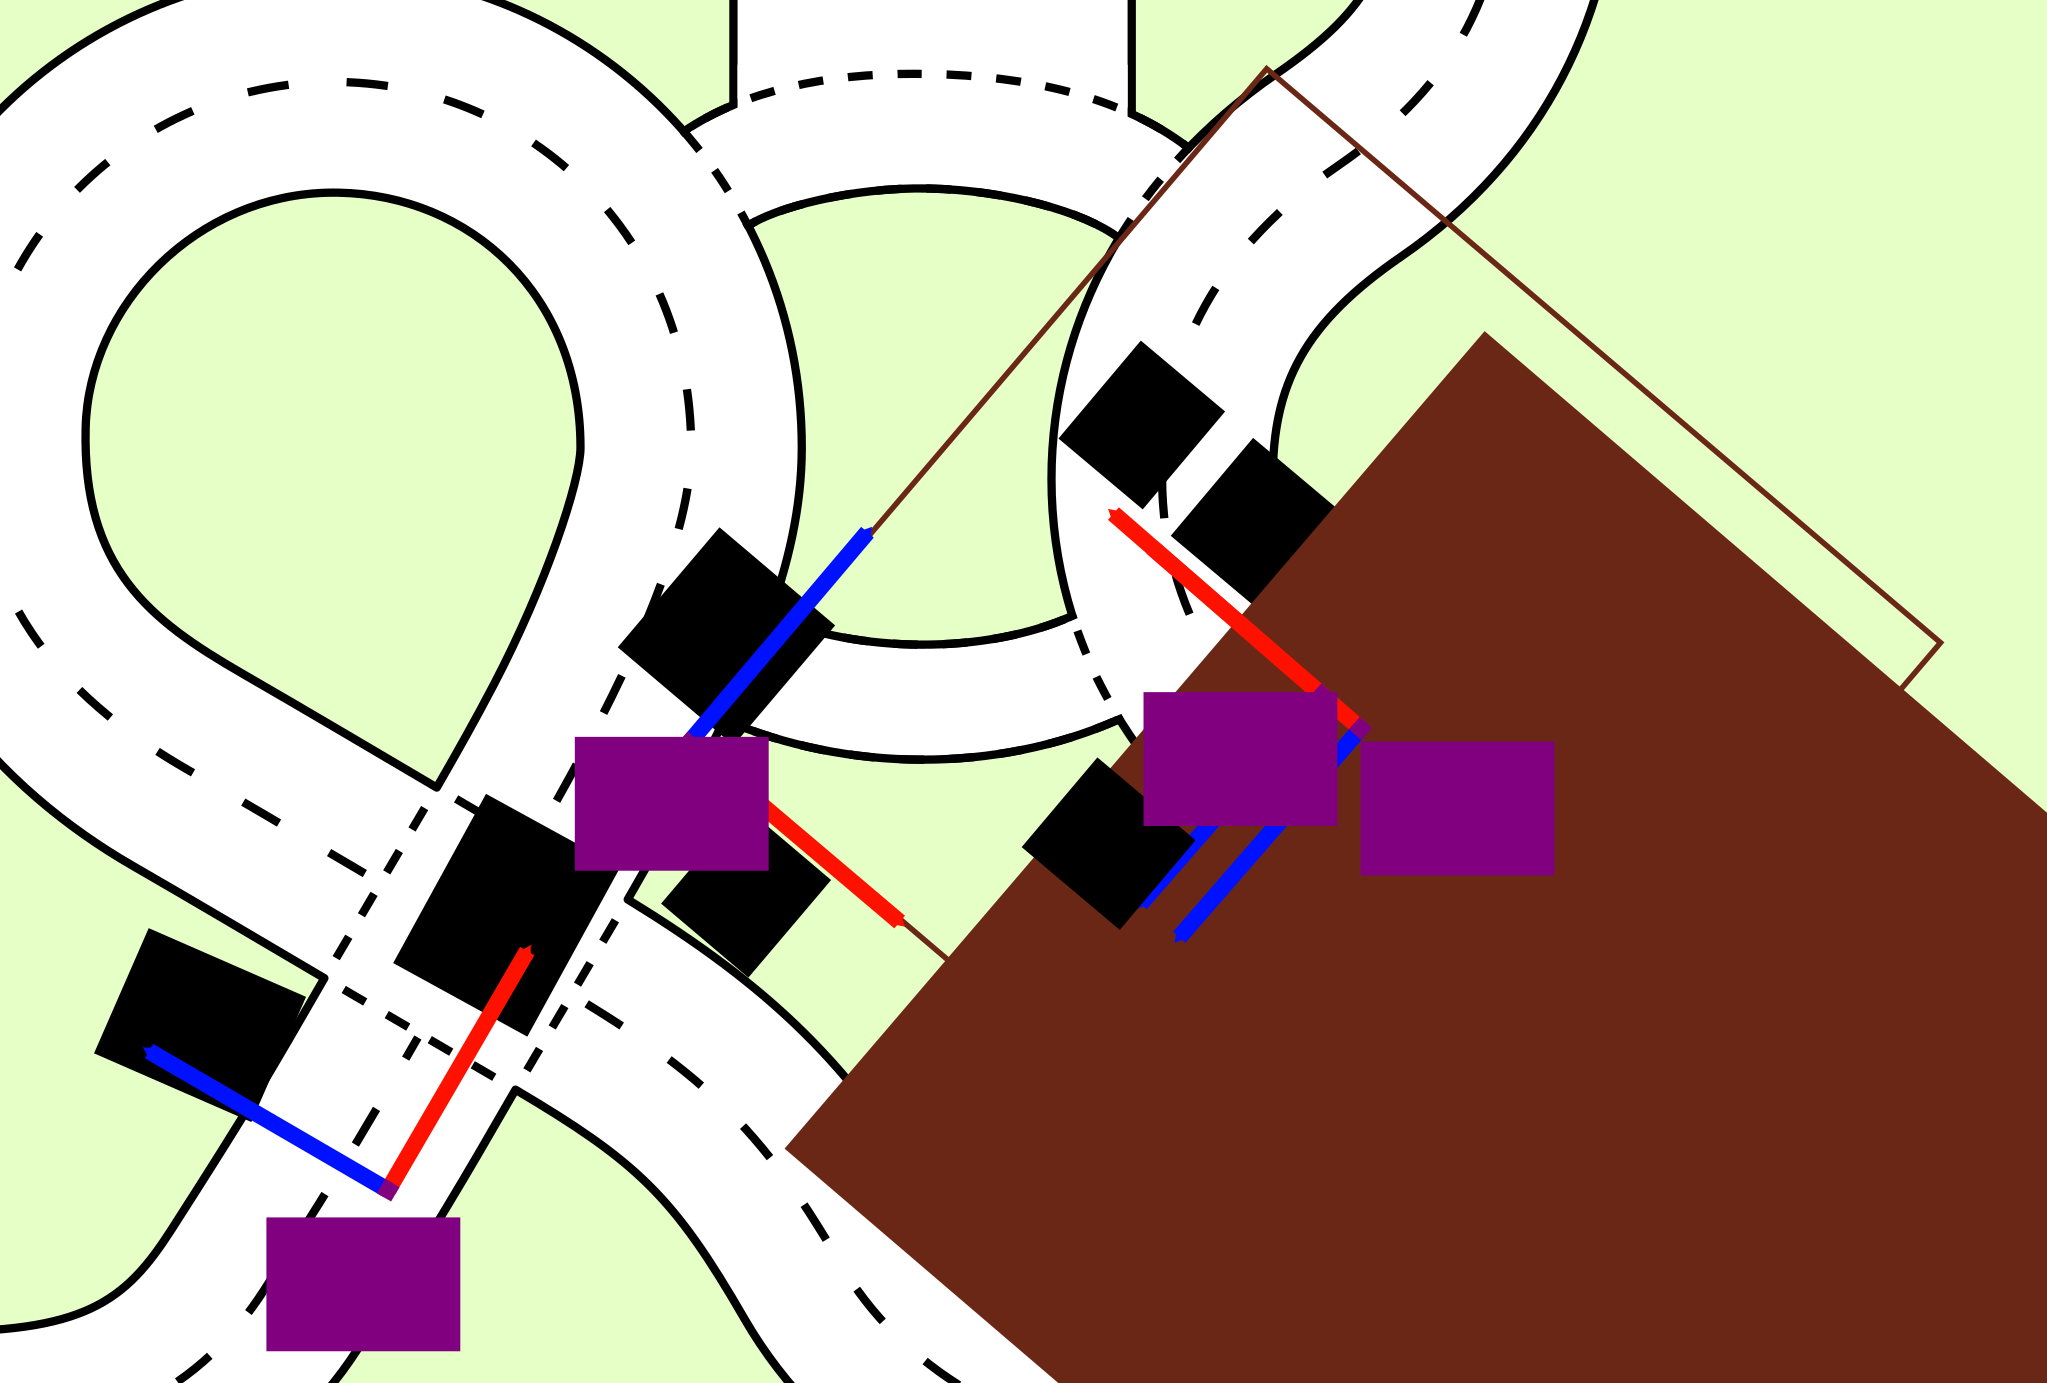
\includegraphics[width=0.9\textwidth]{grundlagen_kos.pdf}
  \caption{Alle eingeführten Koordinatensysteme im Überblick}
  \label{fig:grundlagen_kos}
\end{figure}

Das Weltkoordinatensystem \gls{lat:WeltKOS} bildet die Basis und ist an einem beliebigen Punkt des Szenarios festgemacht. Es dient zur Beschreibung der Pose des mobilen Roboters und der Linienpunkte in der Weltkarte. Damit sich die Pixelkoordinaten nicht von der Matrixindizierung unterscheiden, wird das Bildkoordinatensystem \gls{lat:BildKOS} in die linke obere Ecke des entzerrten Fotos gelegt. So zeigt die x-Achse in Richtung der Zeilen und die Spalten sind gleich der y-Koordinate. In der Hinterachse des Autos liegt das Roboterkoordinatensystem \gls{lat:RoboterKOS}, welches in der Lage zum Weltkoordinatensystem die Pose darstellt.

Um einen Punktvektor \( \gls{lat:Punktvektor}^{\gls{lat:BildKOS}} \) in ein anderes Koordinatensystem zu transformieren, bedarf es einer Verschiebung (Translation) in Richtung eines Verschiebungsvektors \gls{lat:Translationsvektor} und einer Drehung \gls{lat:Rotationsmatrix} (Rotation) um eine Achse. Da sich unser Roboter nur in der xy-Ebene bewegt, wird hier also nur um die z-Achse gedreht.  
Mathematisch lassen sich der Translationsvektor \gls{lat:Translationsvektor} und die Rotationsmatrix \gls{lat:Rotationsmatrix} wie folgt darstellen \autocite{bajdRobotics2010}.

% Formel für den Translationsvektor t
\begin{equation}
\gls{lat:Translationsvektor} = 
\begin{pmatrix}
a 	\\
b 	\\
c    	\\
\end{pmatrix}
, \qquad
% Formel für R = Rot(z,\theta) //(Rotationsmatrix)
\gls{lat:Rotationsmatrix} = Rot(\vec{z},\theta) = 
\begin{pmatrix}
\cos{\theta} & -\sin{\theta} & {0} 	\\
\sin{\theta} & \cos{\theta} & {0} 	\\
{0} & {0} & {1} 				    	\\
\end{pmatrix}
\end{equation} 		

Die Matrix \gls{lat:Transformationsmatrix}, welche die Punkte \gls{lat:Punktvektor} transformiert, sodass 
\( \gls{lat:Punktvektor}_{K_2} = \gls{lat:Transformationsmatrix}^{K_2K_1} \times  \gls{lat:Punktvektor}_{K_1}	\) gilt, heißt homogene Transformationsmatrix und wird folgendermaßen aufgestellt:

% Formel für die Transformationsmatrix T
\begin{equation}
\gls{lat:Transformationsmatrix} = 
\begin{pmatrix}
\gls{lat:Rotationsmatrix} &  \gls{lat:Translationsvektor}	\\
0 \quad 0 \quad 0 & 1 	\\
\end{pmatrix}
=
\begin{pmatrix}
\cos{\theta} & -\sin{\theta} & {0} & a 	\\
\sin{\theta} & \cos{\theta} & {0} & b 	\\
{0} & {0} & {1} & c 				    	\\
0 & 0 & 0 & 1 						\\
\end{pmatrix}
\end{equation}

Den zu transformierenden Punkten muss dazu noch eine Zeile mit einer \(1\) hinzugefügt werden, sonst würden die Dimensionen für die Multiplikation nicht zueinander passen. Sind beispielsweise die Weltkoordinaten von Punkten im Roboterkoordinatensystem gesucht, so stellen \gls{lat:Translationsvektor} die Position und \gls{lat:Orientierung} die Orientierung des Modellfahrzeugs dar. Außerdem gilt: 

% Formel für die Hintereinanderausführung der Transformation
\begin{equation}
\gls{lat:Transformationsmatrix}^{\gls{lat:WeltKOS} \gls{lat:BildKOS}} = 
\gls{lat:Transformationsmatrix}^{\gls{lat:WeltKOS} \gls{lat:RoboterKOS}} \times
\gls{lat:Transformationsmatrix}^{\gls{lat:RoboterKOS} \gls{lat:BildKOS}}
\end{equation}

Sind die einzelnen homogenen, aufeinanderfolgenden Transformationsmatrizen einmal aufgestellt, lassen sich durch deren Matrixmultiplikation die noch Fehlenden bilden. Soll in die umgekehrte Richtung transformiert werden, muss die Inverse der Transformationsmatrix genommen werden. Ein Beispiel für die Transformation des Punktes \( \gls{lat:Punktvektor}^{\gls{lat:RoboterKOS}} \) in Weltkoordinaten sieht dann so aus:

% Beispielformel


